\documentclass{book}
\usepackage[T1]{fontenc}
%\usepackage[standard-baselineskips]{cmbright}
\usepackage{cmbright}
\def\usedfonts{CM-Bright}
\usepackage{graphicx} % includegraphics
\usepackage[numbers]{natbib}     % bibliography style
\begin{document}
%=========================================================================
\section*{Status}
%=========================================================================
\begin{itemize}
\item[Oct. 2015:] The G2 data base has been changed substantially
  again on Oct. 14, 2015. Now the species files are in the nodeless
  construction and the comparison with Paier were good except for
  Na. A number of new tools have been added.
%
\item[Aug 2014:] The G2 data base has been changed substantially on
  Aug. 17, 2014 in order to concentrate the required shell scripts
  into few and to exploit the new paw scripts such as paw\_resolve.
%
\end{itemize}

%=========================================================================
\section*{Overview}
%=========================================================================
\begin{enumerate}
\item \verb+src/g2_makedo+ scans the directory
  \verb+src/Strcfiles+. For each molecule in this directory it creates
  the directories in the directory ``Cases'', if necessary, and it
  creates a shellscript \verb|g2_do_sample|,
\item \verb|g2_do_sample| performs PAW on all molecules. It can be
  added to exclude certain molecules.
\item \verb+src/g2_analyse+ compiles and runs the fortran program
  \verb|src/analyze.f90|, which extracts atomization energies and
  compares them with internal tables of experiment and other numbers.
  It creates a list \verb+readpaw.in+ of the latest energies for all
  molecules, from which it computes the results which are printed in
  in \verb|readpaw.out| in humnan readable form. Some results are
  written to \verb+g2results.dat+ to be viewed with a viewer such as
  \verb|xmgrace|.
\end{enumerate}

%=========================================================================
\section*{Files required}
%=========================================================================
\begin{verbatim}
src/Strcfiles         
src/Speciesfiles      
src/g2_makedo         
src/g2_analyse         
src/g2_analyse.f90       
src/sample.cntl_relax 
src/sample.cntl_start
src/g2_tar
src/splitspecieslist.f90       
src/modify
doc/readme.tex
\end{verbatim}

\begin{itemize}
%
\item \textbf{doc/readme.tex, doc/Figs, doc/Bib, doc/Sources}: documentation of
  the G2-directory.  
%
\item \textbf{Samples/*.strc\_sample}: containes the structure files
  for all molecules without the specific setup information. This
  information will be incorporated into the structure files of all
  calculations.
%
\item \textbf{specieslist}: contains the setup information
  for all elements, which will be included into the structure files.
%
\item \textbf{src/g2\_makedo:} Basic installation and update script:
  \begin{itemize}
     \item Constructs the sample runscript \verb+g2_do_sample+. 
     \item sets up the directory Cases holding the run directories for all
        substances in the \verb|src/Strcfiles| directory.
     \item updates the .strc files for all substances
    \end{itemize}
%
\item \textbf{src/sample.cntl\_start, src/sample.cntl\_relax:} 
    contains the examples for the control input file. 
%
\item \textbf{src/g2\_analyse} shell script to compile and execute
\verb|src/g2_analyse|. It reads readpaw.in and produces readpaw.out.
%
\item \textbf{src/g2\_analyse.f90} fortran code, extracts atomization
  energies and comparison with benchmark tests
%
\item \textbf{src/splitspecies.f90} fortran code, used by
  \verb|src/g2_makedo| to expand the specieslist into separate files.
%
\item \textbf{src/modify} is a small helper script which is not
  required. It may be useful for an administrator to construct scripts
  that perform global changes on a large set of files in one shot.
%
\item \textbf{src/cleanup} is a small helper script which removes some
  of the files in the directory \verb|Cases|, which need not be stored
  permanently.
%
\item \textbf{src/g2\_tar} creates a tar file \verb|bare_g2.tgz|
  containing only the essential files of the database without any
  results.
\end{itemize}

%=========================================================================
\section*{Adapt and run G1 tests}
%=========================================================================
\begin{enumerate}
\item enter the main directory of the database. Check if you are in
  the correct place:
  \begin{itemize} 
    \item execute \verb|ls|. You should obtain ``\verb|src doc|. 
    \item execute \verb|ls src|. You should obtain ``Strcfiles,
      specieslist, g2\_makedo, sample.cntl\_start,
      sample.cntl\_relax, g2\_analyse, g2\_analyse.f90, splitspecies, 
      modify, g2\_cleanup g2\_tar''
   \end{itemize}
%
\item compile this documentation file readme.pdf as follows:
\begin{verbatim}
cd doc
cat Bib/* > all.bib
pdflatex readme
bibtex readme
pdflatex readme
cd ..
\end{verbatim}
%
\item execute \verb|src/g2_makedo|. When done, there should be a
  directory ``\verb|Cases|'' and a shell script ``\verb|g2_do_sample|''
%
\item Adjust the variable NNODES in ``\verb|g2_do_sample|'' to the
  maximum number of paw-related jobs you want to allow on your
  computer.
%
\item make a copy of the shell script \verb|g2_do_sample| with name
  \verb|g2_do| and adjust ``LIST'' in \verb|g2_do| by removing lines
  with those substances that shall be excluded from the calculation.
%
\item create a file \verb|sample.cntl|. One can copy a one of the
  files \verb|src/sample.cntl_start|, \verb|src/sample.cntl_rlxe|, or
  \verb|src/sample.cntl_rlxr| into the current directory and modify
  it. This is the control file used for all calculations.
%
\item execute \verb|g2_do|
%
\end{enumerate}

%=========================================================================
\subsection*{Construct documentation}
%=========================================================================

\begin{verbatim}
cd doc
cat Bib/* > all.bib
pdflatex readme
bibtex readme
pdflatex readme
\end{verbatim}


%=====================================================
\section*{Problems}
%=====================================================
\begin{itemize}
\item Some of the atoms cannot be converged with Safeortho=F because of 
its energy-level structure
\item The hydrogen atom has problems probably because there is no spin
density in the minority spin direction. NO! it seems to be also
safeortho. Again YES: I get problems also with SAFEORTHO=T. It helps
to make a calculation with spin[hbar]=0.499 and then multiply the
energy level difference with 0.001. 
\begin{center}
\includegraphics[width=0.5\linewidth,clip=t]{Figs/hydrogenetot.eps}
\begin{tabular}{|l|r|r|r|}
\hline
$\frac{1}{2}\hbar-S$ & $E_{tot}[H]$ & $\epsilon_\uparrow$[eV]& $\epsilon_\downarrow$[eV] \\
\hline
0.001 &  -0.4984656 &  -7.621&   -0.388 \\
0.005 &  -0.4974234 &  -7.646&   -0.627\\ 
0.010 &  -0.4961265 &  -7.686&   -0.831 \\
0.020 &  -0.4935614 &  -7.766&   -1.091 \\
\hline
\end{tabular}
\end{center}
\begin{eqnarray*}
E_{tot}[H]=-0.49872+0.258(\frac{1}{2}-S/hbar)
\end{eqnarray*}
If we perform calculations with a spin of $0.4990 \hbar$, the total
energy is too high by $0.2544\times 10^3$~H.

The unit cell for hydrogen has been fixed to a lattice constant of
10~\AA to avoid instabilitis.

\item Be2 may need a larger cell!
\item take care of zero point vibration energy
\item in DFT some of the atoms are non-psherical
\item The G2 database contains some open shell systems besides atoms:
BeH (spin=0.5$\hbar$), CH,\ldots
\begin{itemize}
\item C$_2$ is has a band crossing of a $\sigma$-state and a doublet of
$\pi$ states right at the energy minimum
\end{itemize}
\item for Li I had to reduce the projectors with the nodeless
  setups to npro=1 0 0 to avoid an instability. This is probably
  the well-known overcompleteness problem.
\end{itemize}

%=========================================================================
\newpage
\section*{Results}
%=========================================================================

%=========================================================================
\subsection*{Benchmark Oct.17, 2015}
%=========================================================================
Look up the paw\_setups report for a systematic study of constructing a
set of species.

\begin{itemize}
\item O-cutoff: $r_{c,\ell}=0.75\;r_{cov}$. Oxygen is the most
  critical element with one of the slowest plane wave convergence. It
  is the smallest first row element (following Ne and F) which in
  addition forms strong bonds. Furthermore it is a ubiquitous
  element. With this cutoff the O$_2$ bondlength deviates by less than
  1~\%. The result can be improved with a cutoff of
  $r_{c,\ell}=0.75\;r_{cov}$ at the cost of a slower plane wave
  convergence.
%
\item H-cutoff: $r_{c,\ell}=1.2\;r_{cov}$. Hydrogen is a frequent
  element. It does not have any core states so that the partial waves
  turn into all-electron wave functions if the cutoff is reduced.
%
\item C-cutoff: $r_{c,\ell}=0.75\;r_{cov}$. Compounds with oxygen, CO
  and CO$_2$ gave results that vary a lot with $r_{c,\ell}$. At the
  chosen value the energies go through a minimum so that the results
  are maximally independent of the cutoff.
%
\item N-cutoff: $r_{c,\ell}=0.75\;r_{cov}$. Nitrogen forms very strong
  bonds and is intermediate of oxygen and carbon. Therefore it is
  treated similarly.
%
\item Other first-row elements with p-electrons
  $r_{c,\ell}=0.75\;r_{cov}$.  We choose the other first-row elements
  with p-electrons similar to C,N and O.
%
\item first-row elements with s-electrons $r_{c,\ell}=0.85\;r_{cov}$.
  Lithium and beryllium obtain a somwhat larger radius. (No special reason)
%
\item second-row elements with p-electrons $r_{c,\ell}=0.9\;r_{cov}$.
\end{itemize}

\includegraphics[width=\linewidth]{Figs/151017_Benchmark/151017_benchmark}

Problems:
\begin{itemize}
\item The Na setup is defunct
\item the Br setup is defunct
\item 86(Cl$_2$), 89 (ClO) and (98) FCl deviate more than 0.1~eV
  beyond the VASP, GAUSS and GPAW calculations. This indicates that the
  Cl setup is not very good.
\item the atomic structure has not been relaxed in the test.
\item the deviations are more on the negative. This could be a sign
  that the results improve with a larger plane wave cutoff, or after
  relaxing the atomic positions
\end{itemize}


%=========================================================================
\subsection*{Benchmark Oct.10, 2015}
%=========================================================================
Test nodeless setups using the PBE
functional\cite{perdew96_prl77_3865}. The comparison has been done on
the basis of the G2 database. The comparison has been done with the
calculations using VASP and Gaussian by Paier et
al.\cite{paier05_jcp122_234102}


\begin{figure}[h!]
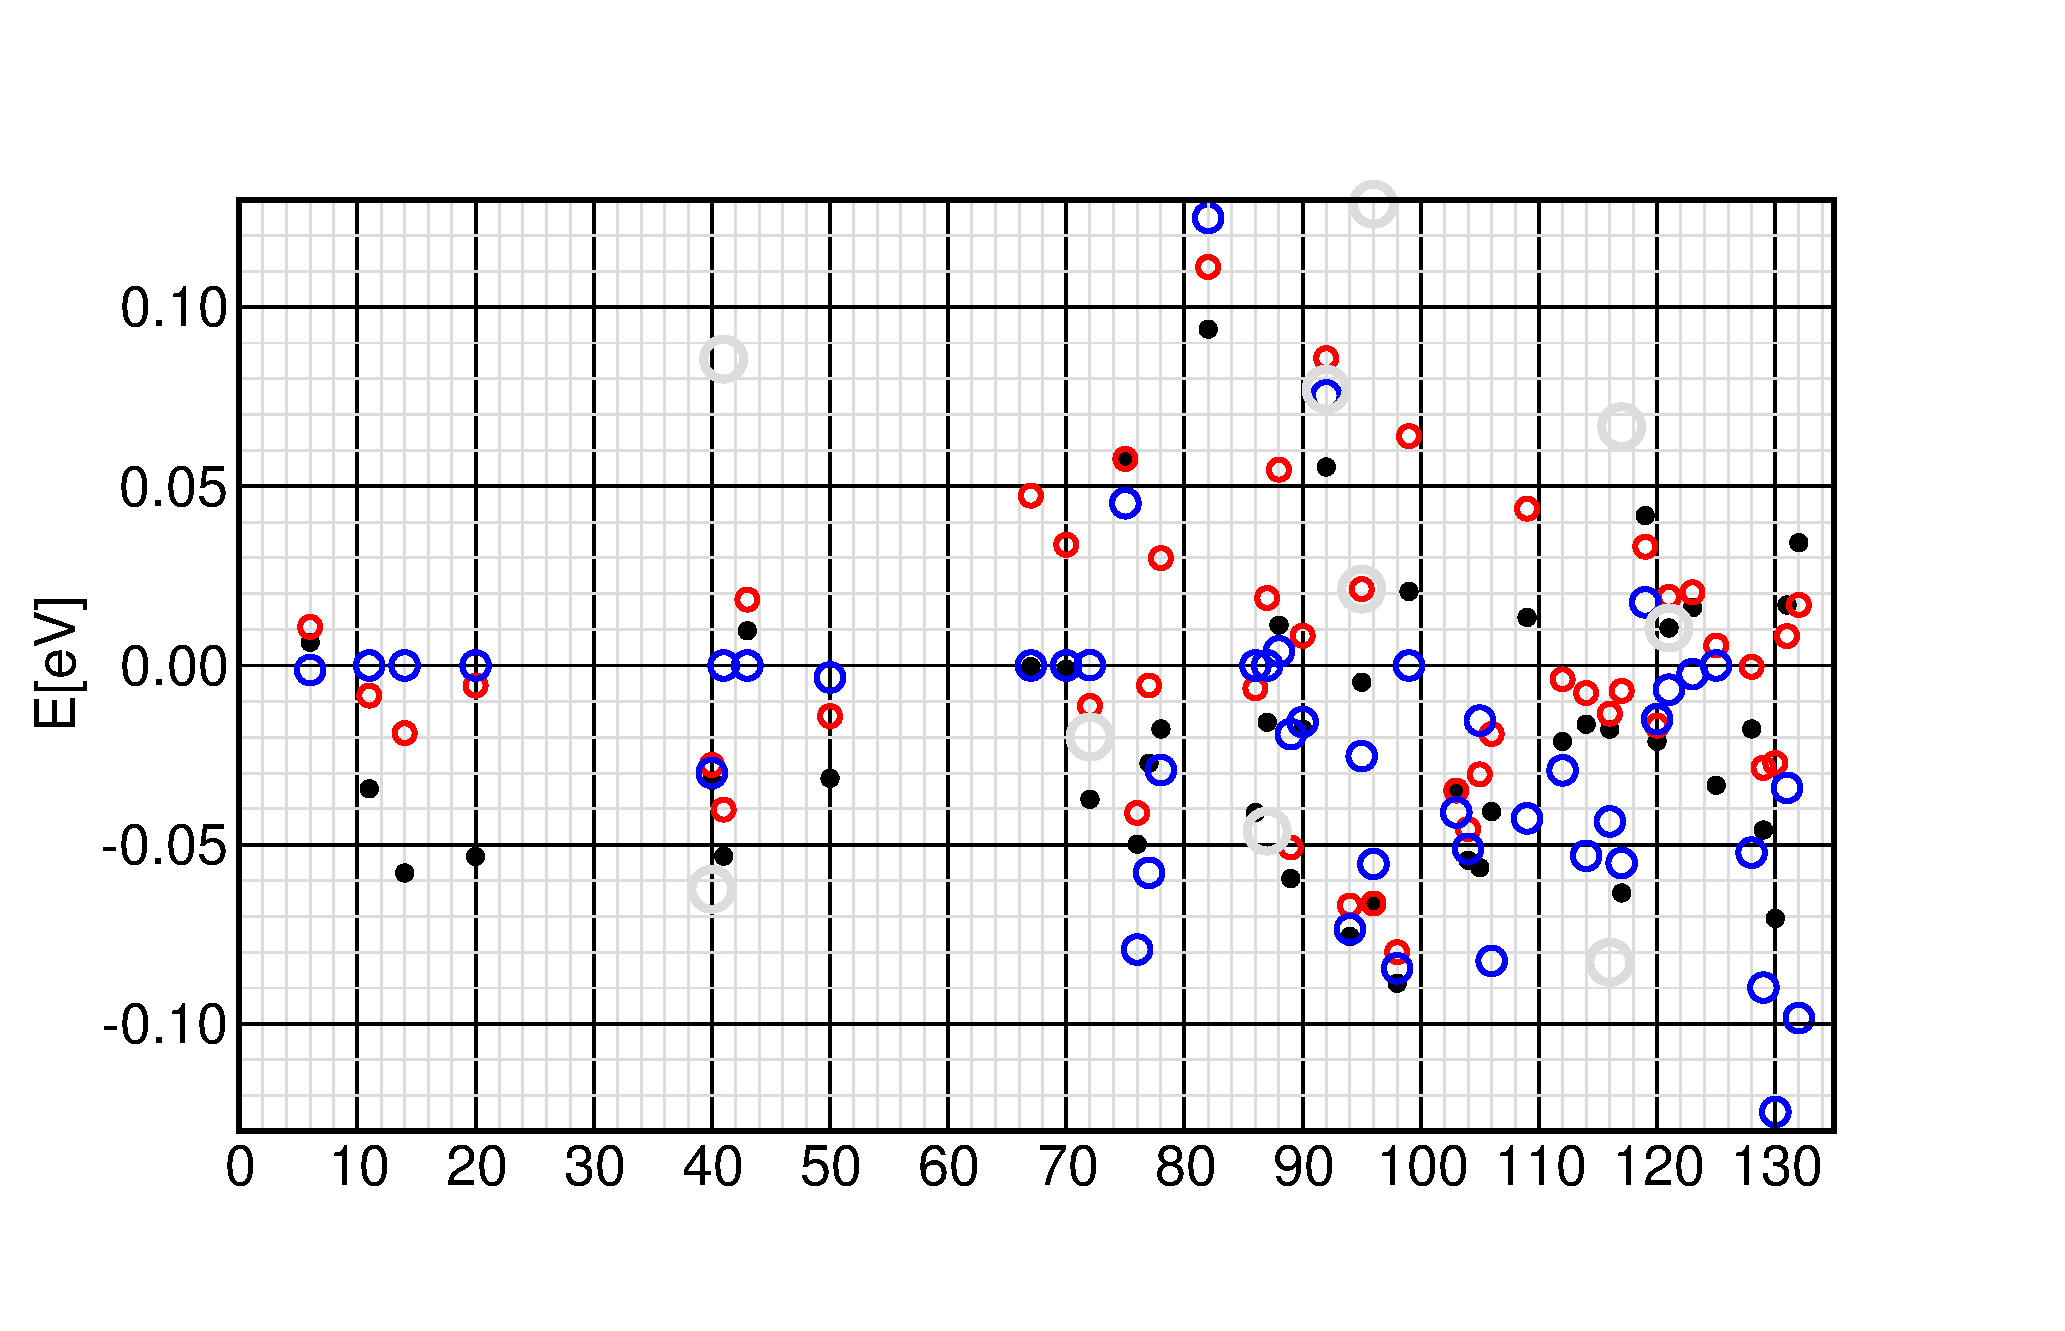
\includegraphics[width=\linewidth]{Figs/151010benchmark/g2benchmark}
\caption{\label{fig:151010benchmark}Deviations of atomization energies
  calculated by VASP (black dots), Gaussian (red spheres) and GPAW
  (blue spheres) from CPPAW and obtained from experiment. The largest
  consisten deviations are for F$_2$ (82), HF (92),Li$_2$ (94), LiH
  (96) and N$_2$ (98). }
\end{figure}

{\tiny
\begin{verbatim}
!CONTROL
 !GENERIC NSTEP=200 DT=10.0 NWRITE=100 START=F  !END 
 !FOURIER EPWPSI=80. CDUAL=4.0 !END
 !DFT     TYPE=10 !END 
 !PSIDYN STOP=T  FRIC=0.05 
   !AUTO FRIC(-)=0.05 FACT(-)=0.97  FRIC(+)=0.3 FACT(+)=1. minfric=0.01 !END
 !END
!END
!EOB 
\end{verbatim}
}

Below, the setup parameters are provided. Note, that the NTBO
construction is not used.
{\tiny
\begin{verbatim}
  !SPECIES   NAME='Al'  M=40. NPRO=2 2 1 LRHOX=4 RAD/RCOV=1.0
    !NTBO    NOFL=1 1 0 CV=T LHFWEIGHT=0.100
             TAILLAMBDA=4.0 2.0 RAUG/RCOV=1.2 RTAIL/RCOV=1.4 
    !END 
    !AUGMENT ID='MY_NDLSS_AL' EL='AL' ZV= 3.
             TYPE='NDLSS' RBOX/RCOV=1.2 RCSM/RCOV=.25
             RCL/RCOV=.919 .919 .919 .919
      !GRID  DMIN=1.E-6 DMAX=.15 RMAX=9. !END
      !POT   POW=3. RC/RCOV=.919 VAL0_X= -1.5 !END
      !CORE  POW=2. RC/RCOV=.919 !END
    !END
  !END
  !SPECIES   NAME='B_'  M=40. NPRO=1 1 1 LRHOX=4 RAD/RCOV=1.4
    !NTBO    NOFL=1 1 0 CV=T LHFWEIGHT=0.100
             TAILLAMBDA=4.0 2.0 RAUG/RCOV=1.2 RTAIL/RCOV=1.4 
    !END 
    !AUGMENT ID='MY_NDLSS_B' EL='B' ZV= 3.
             TYPE='NDLSS' RBOX/RCOV=1.2 RCSM/RCOV=.25
             RCL/RCOV=.75 .75 .75 .75
      !GRID  DMIN=1.E-6 DMAX=.15 RMAX=9. !END
      !POT   POW=3. RC/RCOV=.774 VAL0_X= -3.9 !END
      !CORE  POW=2. RC/RCOV=.774 !END
    !END
  !END
  !SPECIES   NAME='BE'  M=40. NPRO=1 1 0 LRHOX=2 RAD/RCOV=1.4
    !NTBO    NOFL=1 1 0 CV=T LHFWEIGHT=0.100
             TAILLAMBDA=4.0 2.0 RAUG/RCOV=1.2 RTAIL/RCOV=1.4 
    !END 
    !AUGMENT ID='MY_NDLSS_BE' EL='BE' ZV= 2.
             TYPE='NDLSS' RBOX/RCOV=1.2 RCSM/RCOV=.25
             RCL/RCOV=.882 .882 .882 .882
      !GRID  DMIN=1.E-6 DMAX=.15 RMAX=9. !END
      !POT   POW=3. RC/RCOV=.882 VAL0_X= -1.6 !END
      !CORE  POW=2. RC/RCOV=.882 !END
    !END
  !END
  !SPECIES   NAME='Br'  M=40. NPRO=1 1 1 LRHOX=2 RAD/RCOV=1.4
    !NTBO    NOFL=1 1 0 CV=T LHFWEIGHT=0.100
             TAILLAMBDA=4.0 2.0 RAUG/RCOV=1.2 RTAIL/RCOV=1.4 
    !END 
    !AUGMENT ID='MY_NDLSS_BR' EL='BR' ZV= 7.
             TYPE='NDLSS' RBOX/RCOV=1.2 RCSM/RCOV=.25
             RCL/RCOV=.975 .975 .975 .975
      !GRID  DMIN=1.E-6 DMAX=.15 RMAX=9. !END
      !POT   POW=3. RC/RCOV=.975 VAL0_X= -2.0 !END
      !CORE  POW=2. RC/RCOV=.975 !END
    !END
  !END
  !SPECIES   NAME='C_'  M=40. NPRO=1 1 1 LRHOX=4 RAD/RCOV=1.4
    !NTBO    NOFL=1 1 0 CV=T LHFWEIGHT=0.100
             TAILLAMBDA=4.0 2.0 RAUG/RCOV=1.2 RTAIL/RCOV=1.4 
    !END 
    !AUGMENT ID='MY_NDLSS_C' EL='C' ZV= 4.
             TYPE='NDLSS' RBOX/RCOV=1.2 RCSM/RCOV=.25
             RCL/RCOV=0.85 0.85 0.85 0.85 
      !GRID  DMIN=1.E-6 DMAX=.15 RMAX=9. !END
      !POT   POW=3. RC/RCOV=0.75  VAL0_X=-2.7 !END
      !CORE  POW=2. RC/RCOV=0.75  !END
    !END
  !END
  !SPECIES   NAME='CL'  M=40. NPRO=2 2 1 LRHOX=2 RAD/RCOV=1.4
    !NTBO    NOFL=1 1 0 CV=T LHFWEIGHT=0.100
             TAILLAMBDA=4.0 2.0 RAUG/RCOV=1.2 RTAIL/RCOV=1.4 
    !END 
    !AUGMENT ID='MY_NDLSS_CL' EL='CL' ZV= 7.
             TYPE='NDLSS' RBOX/RCOV=1.2 RCSM/RCOV=.25
             RCL/RCOV=0.802 0.802 0.802 0.802 
      !GRID  DMIN=1.E-6 DMAX=.15 RMAX=9. !END
      !POT   POW=3. RC/RCOV=0.802 VAL0_X=-3.5 !END
      !CORE  POW=2. RC/RCOV=0.802  !END
    !END
  !END
  !SPECIES   NAME='F_'  M=80. NPRO=1 1 1 LRHOX=2 RAD/RCOV=1.4
    !NTBO    NOFL=1 1 0 CV=T LHFWEIGHT=0.100
             TAILLAMBDA=4.0 2.0 RAUG/RCOV=1.2 RTAIL/RCOV=1.4 
    !END 
    !AUGMENT ID='MY_NDLSS_F' EL='F_' ZV= 7.
             TYPE='NDLSS' RBOX/RCOV=1.2 RCSM/RCOV=.25
             RCL/RCOV=0.8 0.8 0.8  0.8 
      !GRID  DMIN=1.E-6 DMAX=.15 RMAX=9. !END
      !POT   POW=3. RC/RCOV=0.75 VAL0_X=-3.5 !END
      !CORE  POW=2. RC/RCOV=0.75  !END
    !END
  !END
  !SPECIES   NAME='H_'  M=2. NPRO=1 1 LRHOX=2 RAD/RCOV=1.2
    !NTBO    NOFL=1 0 CV=T LHFWEIGHT=0.100
             TAILLAMBDA=4.0 2.0 RAUG/RCOV=1.2 RTAIL/RCOV=1.4 
    !END 
    !AUGMENT ID='MY_NDLSS_H' EL='H' ZV= 1.
             TYPE='NDLSS' RBOX/RCOV=1.2 RCSM/RCOV=.25
             RCL/RCOV=1.2 1.2  1.2  1.2 
      !GRID  DMIN=1.E-6 DMAX=.15 RMAX=9. !END
      !POT   POW=3. RC/RCOV=1.2 VAL0_X=-1.6 !END
      !CORE  POW=2. RC/RCOV=1.2 !END
    !END
  !END
  !SPECIES   NAME='LI'  M=40. NPRO=1 0  LRHOX=4 RAD/RCOV=1.0
    !NTBO    NOFL=1 0 0 CV=T LHFWEIGHT=0.100
             TAILLAMBDA=4.0 2.0 RAUG/RCOV=1.2 RTAIL/RCOV=1.4 
    !END 
    !AUGMENT ID='MY_NDLSS_LI' EL='LI' ZV= 1.
             TYPE='NDLSS' RBOX/RCOV=1.2 RCSM/RCOV=.25
             RCL/RCOV=.861 .861 .861  .861 
      !GRID  DMIN=1.E-6 DMAX=.15 RMAX=9. !END
      !POT   POW=3. RC/RCOV=.861 VAL0_X=-0.8 !END
      !CORE  POW=2. RC/RCOV=.861  !END
    !END
  !END
  !SPECIES   NAME='N_'  M=40. NPRO=1 1 1 LRHOX=4 RAD/RCOV=1.4
    !NTBO    NOFL=1 1 0 CV=T LHFWEIGHT=0.100
             TAILLAMBDA=4.0 2.0 RAUG/RCOV=1.2 RTAIL/RCOV=1.4 
    !END 
    !AUGMENT ID='MY_NDLSS_N' EL='N' ZV= 5.
             TYPE='NDLSS' RBOX/RCOV=1.2 RCSM/RCOV=.25
             RCL/RCOV=0.75 0.75 0.75  0.75
      !GRID  DMIN=1.E-6 DMAX=.15 RMAX=9. !END
      !POT   POW=3. RC/RCOV=0.75 VAL0_X=-4.3 !END
      !CORE  POW=2. RC/RCOV=0.75  !END
    !END
  !END
  !SPECIES   NAME='Na'  M=40. NPRO=2 2 1 LRHOX=4 RAD/RCOV=1.0
    !NTBO    NOFL=1 1 0 CV=T LHFWEIGHT=0.100
             TAILLAMBDA=4.0 2.0 RAUG/RCOV=1.2 RTAIL/RCOV=1.4 
    !END 
    !AUGMENT ID='MY_NDLSS_NA' EL='NA' ZV= 9.
             TYPE='NDLSS' RBOX/RCOV=1.2 RCSM/RCOV=.25
             RCL/RCOV=0.780 0.790 0.804
      !GRID  DMIN=1.E-6 DMAX=.15 RMAX=9. !END
      !POT   POW=3. RC/RCOV=0.766 VAL0_X=-1.1  !END
      !CORE  POW=2. RC/RCOV=0.766  !END
    !END
  !END
  !SPECIES   NAME='O_'  M=80. NPRO=1 1 1 LRHOX=4 RAD/RCOV=1.4
    !NTBO    NOFL=1 1 0 CV=T LHFWEIGHT=0.100
             TAILLAMBDA=4.0 2.0 RAUG/RCOV=1.2 RTAIL/RCOV=1.4 
    !END 
    !AUGMENT ID='MY_NDLSS_O' EL='O' ZV= 6.
             TYPE='NDLSS' RBOX/RCOV=1.2 RCSM/RCOV=.25
             RCL/RCOV=.65 0.65 0.65 0.65
      !GRID  DMIN=1.E-6 DMAX=.15 RMAX=9. !END
      !POT   POW=3. RC/RCOV=0.65 VAL0_X=-3.8 !END
      !CORE  POW=2. RC/RCOV=.65 !END
    !END
  !END
  !SPECIES   NAME='P_'  M=40. NPRO=2 2 1 LRHOX=2 RAD/RCOV=1.4
    !NTBO    NOFL=1 1 0 CV=T LHFWEIGHT=0.100
             TAILLAMBDA=4.0 2.0 RAUG/RCOV=1.2 RTAIL/RCOV=1.4 
    !END 
    !AUGMENT ID='MY_NDLSS_P' EL='P_' ZV= 5.
             TYPE='NDLSS' RBOX/RCOV=1.2 RCSM/RCOV=.25
             RCL/RCOV=0.899 0.899 0.899  0.899 
      !GRID  DMIN=1.E-6 DMAX=.15 RMAX=9. !END
      !POT   POW=3. RC/RCOV=.899 VAL0_X=-2.4 !END
      !CORE  POW=2. RC/RCOV=.899 !END
    !END
  !END
  !SPECIES   NAME='S_'  M=40. NPRO=2 2 1 LRHOX=4 RAD/RCOV=1.4
    !NTBO    NOFL=1 1 0 CV=T LHFWEIGHT=0.100
             TAILLAMBDA=4.0 2.0 RAUG/RCOV=1.2 RTAIL/RCOV=1.4 
    !END 
    !AUGMENT ID='MY_NDLSS_S' EL='S_' ZV= 6.
             TYPE='NDLSS' RBOX/RCOV=1.2 RCSM/RCOV=.25
             RCL/RCOV=0.954 0.960  0.882  0.882
      !GRID  DMIN=1.E-6 DMAX=.15 RMAX=9. !END
      !POT   POW=3. RC/RCOV=0.742 VAL0_X=-3.3 !END
      !CORE  POW=2. RC/RCOV=0.742 !END
    !END
  !END
  !SPECIES   NAME='Si'  M=40. NPRO=2 2 1 LRHOX=4 RAD/RCOV=1.4
    !NTBO    NOFL=1 1 0 CV=T LHFWEIGHT=0.100
             TAILLAMBDA=4.0 2.0 RAUG/RCOV=1.2 RTAIL/RCOV=1.4 
    !END 
    !AUGMENT ID='MY_NDLSS_SI' EL='SI' ZV= 4.
             TYPE='NDLSS' RBOX/RCOV=1.2 RCSM/RCOV=.25
             RCL/RCOV=0.953 0.953 0.953 0.953 
      !GRID  DMIN=1.E-6 DMAX=.15 RMAX=9. !END
      !POT   POW=3. RC/RCOV=0.953  VAL0_X= -1.8 !END
      !CORE  POW=2. RC/RCOV=0.953  !END
    !END
  !END
\end{verbatim}
}


\bibliographystyle{unsrtnat}
\bibliography{all}
\end{document}
